\documentclass[10pt,letterpaper]{article}
\usepackage[top=0.5in,footskip=0.5in,left=1.25in,right=1.25in]{geometry}

% amsmath and amssymb packages, useful for mathematical formulas and symbols
\usepackage{amsmath,amssymb}

% Use adjustwidth environment to exceed column width (see example table in text)
\usepackage{changepage}

% Use Unicode characters when possible
\usepackage[utf8x]{inputenc}

% textcomp package and marvosym package for additional characters
\usepackage{textcomp,marvosym}

% cite package, to clean up citations in the main text. Do not remove.
\usepackage{cite}

% Use nameref to cite supporting information files (see Supporting Information section for more info)
\usepackage{nameref,hyperref}

% line numbers
\usepackage[right]{lineno}

% ligatures disabled
\usepackage{microtype}
\DisableLigatures[f]{encoding = *, family = * }

% Bold the 'Figure #' in the caption and separate it from the title/caption with a period
% Captions will be left justified
\usepackage[aboveskip=5px,labelfont=bf,labelsep=period,justification=centering,singlelinecheck=off]{caption}
\renewcommand{\figurename}{Fig S} 

% Header and Footer with logo
\usepackage{graphicx}
\graphicspath{ {./figures/} } % define graphics location


\begin{document}
\vspace*{0.2in}

\begin{center}
{\Huge\textbf{Supporting Figures}}
\end{center}
\vspace*{0.5in}

\begin{figure}[h!]
\centering
\includegraphics[width=1.0\columnwidth]{./figure_S1}
\caption{\textbf{Example clones in the larval fly eye.}}
\end{figure}
\pagebreak

\begin{figure}[h]
\centering
\includegraphics[scale=1.0]{./figure_S2}
\caption{\textbf{Using background pixels to characterize bleedthrough contributions in the foreground.}}
\end{figure}
\pagebreak

\begin{figure}[h]
\centering
\includegraphics[scale=1.0]{./figure_S3}
\caption{\textbf{Training a clone annotation model.}}
\end{figure}
\pagebreak

\begin{figure}[h]
\centering
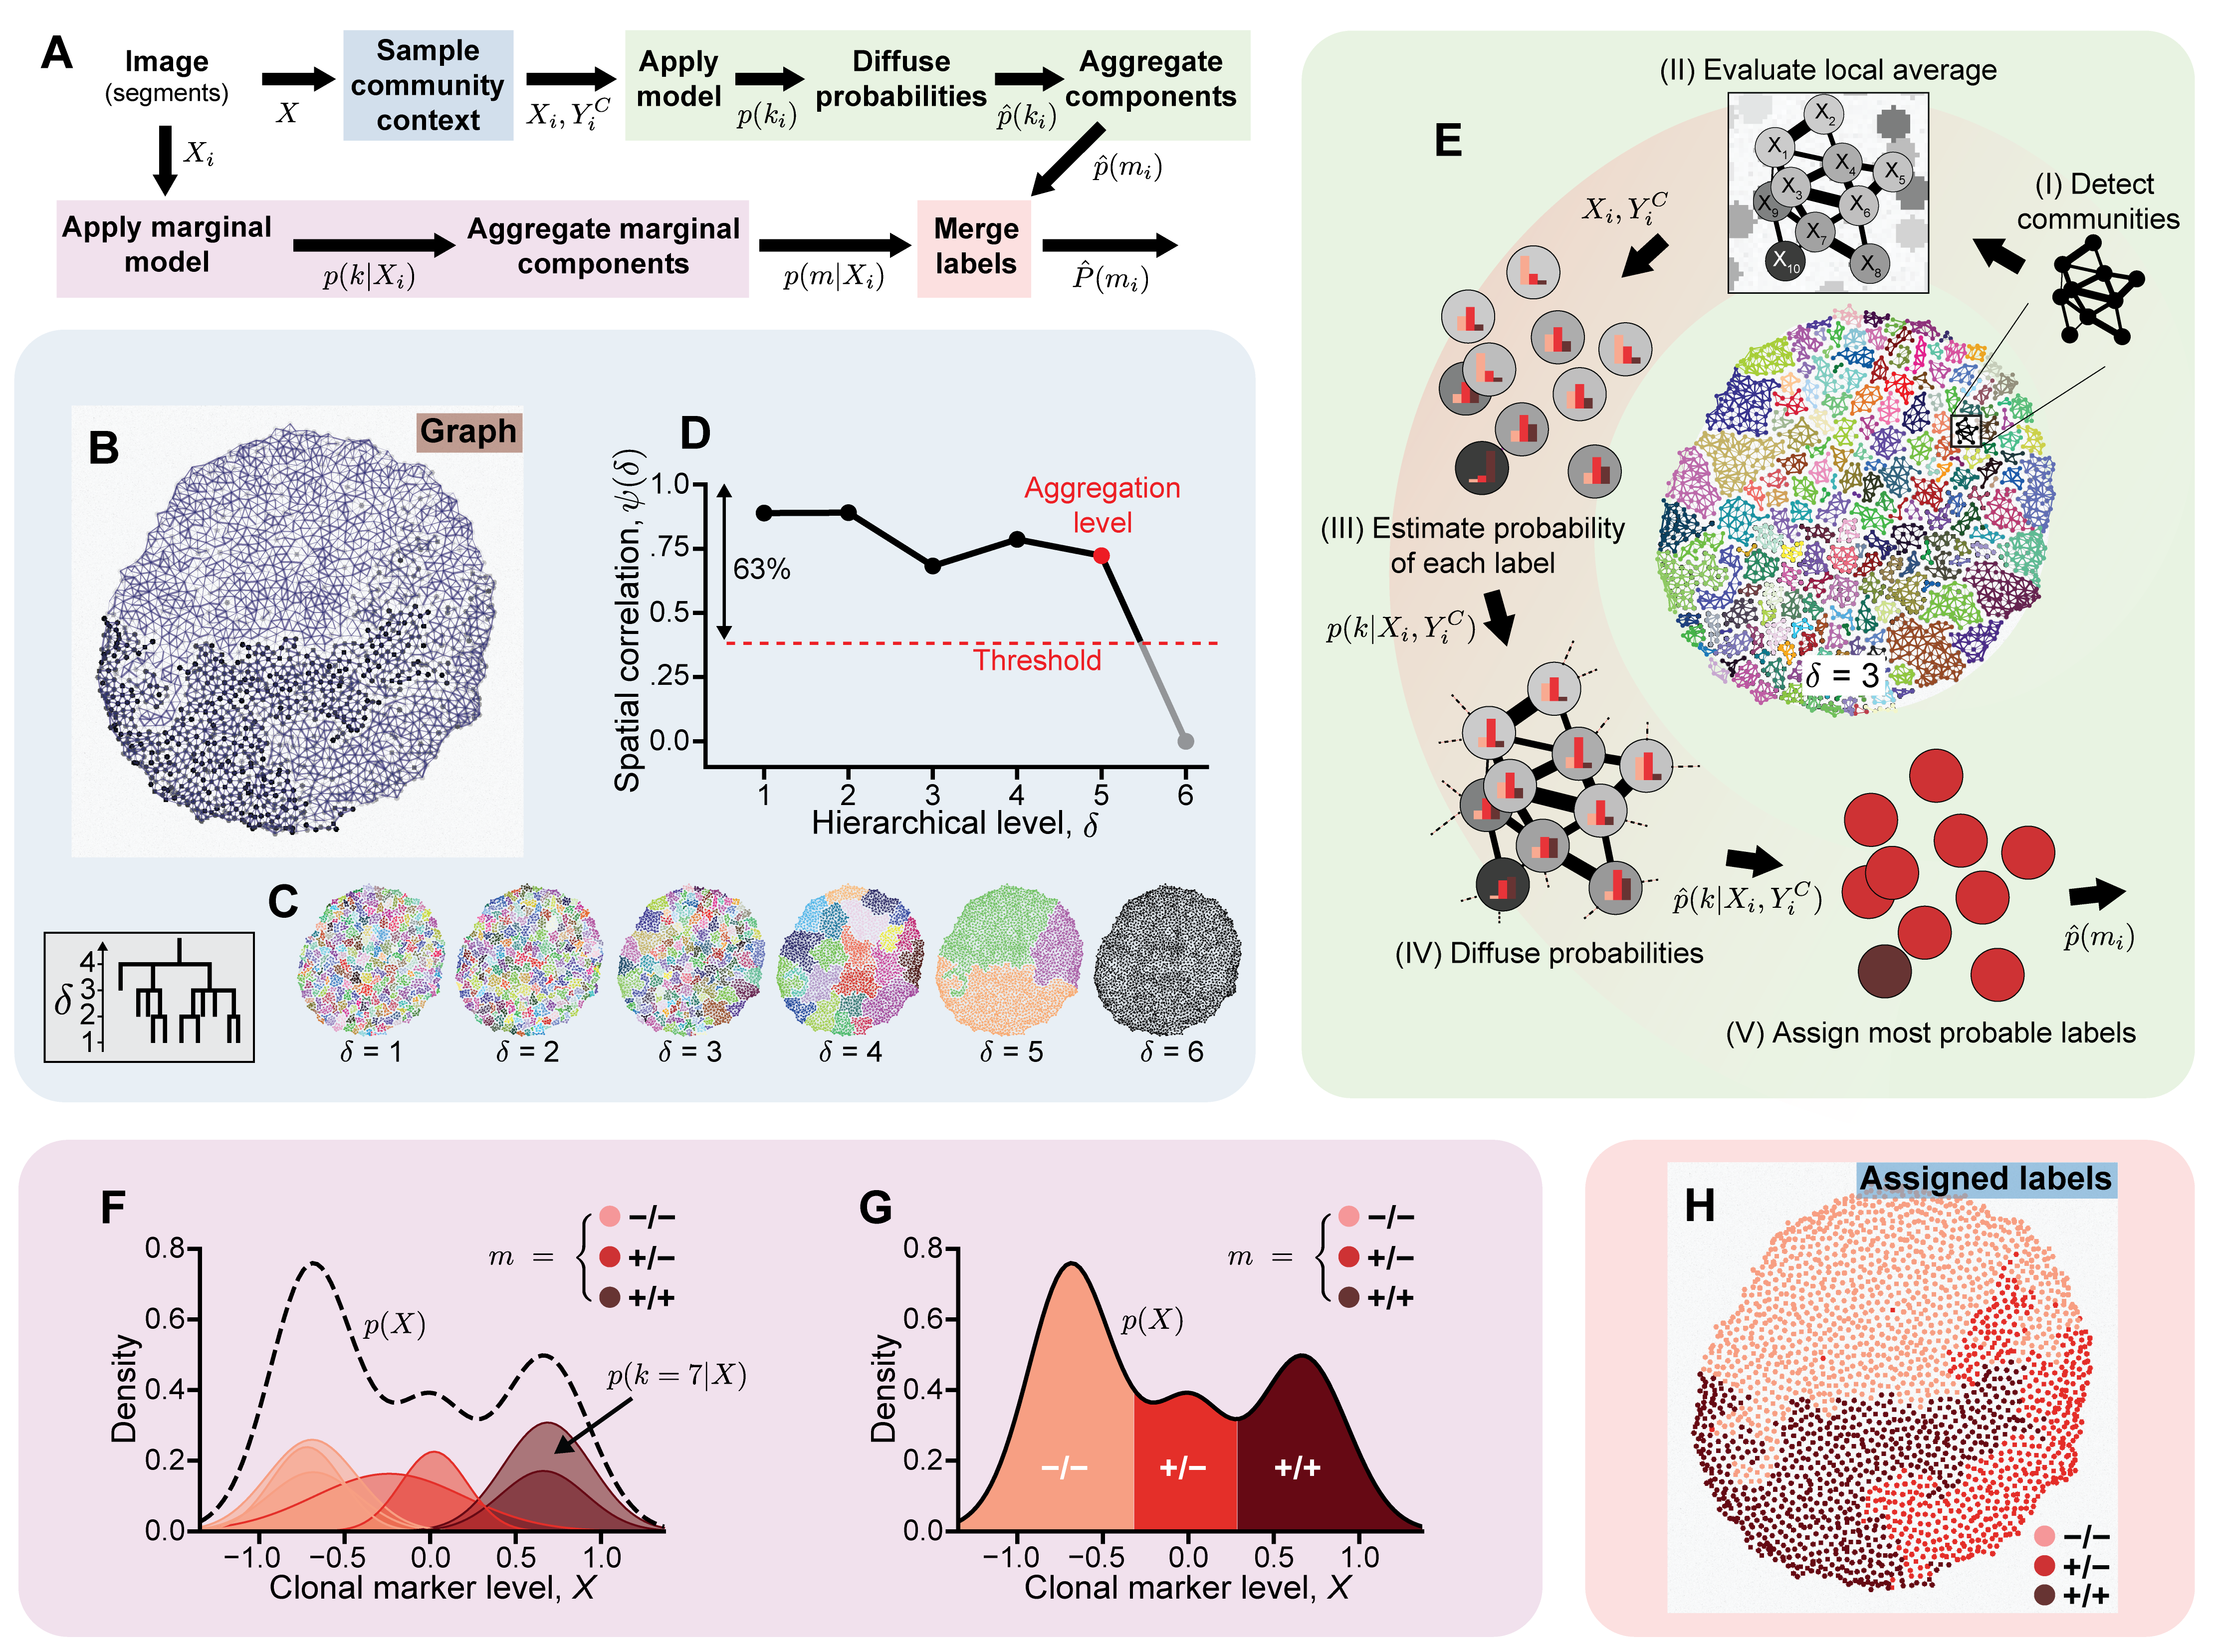
\includegraphics[width=1.0\columnwidth]{./figure_S4}
\caption{\textbf{Label assignment using a trained clone annotation model.}}
\end{figure}
\pagebreak

\begin{figure}[h]
\centering
\includegraphics[scale=1.0]{./figure_S5}
\caption{\textbf{Comparison of automated annotation with manually assigned labels.}}
\end{figure}
\pagebreak

\begin{figure}[h]
\centering
\includegraphics[width=1.0\columnwidth]{./figure_S6}
\caption{\textbf{Simulated growth of a synthetic cell culture.}}
\end{figure}
\pagebreak

\begin{figure}[h]
\centering
\includegraphics[width=1.0\columnwidth]{./figure_S7}
\caption{\textbf{Tunable generation of synthetic microscopy data.}}
\end{figure}
\pagebreak

\begin{figure}[h]
\centering
\includegraphics[scale=1]{./figure_S8}
\caption{\textbf{Spatial context is most informative for large clones with ambiguous fluorescence.}}
\end{figure}

\end{document}
